\section{Results}
In this section we revisit the Prisoners Dilemma model of \cite{nowak_evolutionary_1992} and present the Heroes \& Cowards model of \cite{wilensky_introduction_2015} and show results simulating both with the four update-strategies. 

\subsection{Prisoners Dilemma}
\begin{figure*}
        \centering
        \begin{subfigure}[b]{0.475\textwidth}
            \centering
            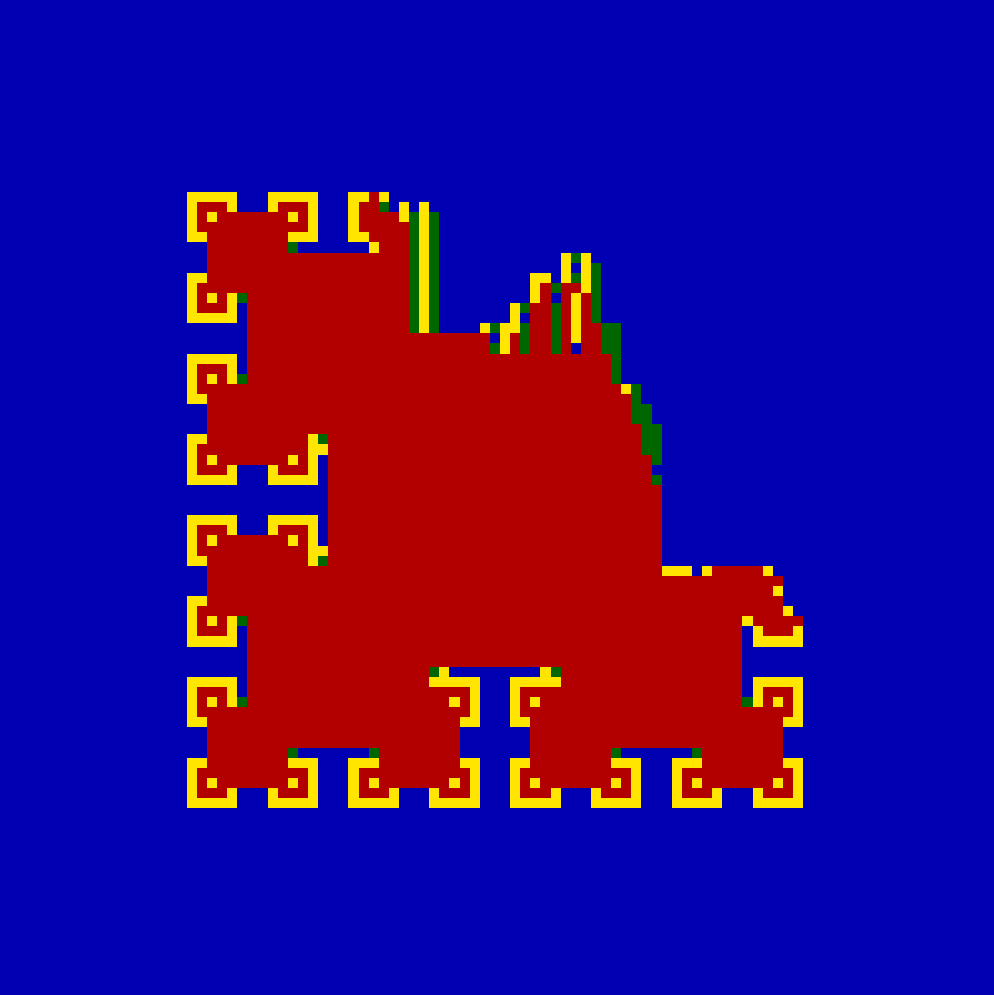
\includegraphics[width=.4\textwidth, angle=0]{./fig/seq_99x99_62steps_MSG_haskell.png}
            \caption[]%
            {{\small Sequential Strategy}}    
            \label{fig:seq_strat}
        \end{subfigure}
        \hfill
        \begin{subfigure}[b]{0.475\textwidth}  
            \centering 
            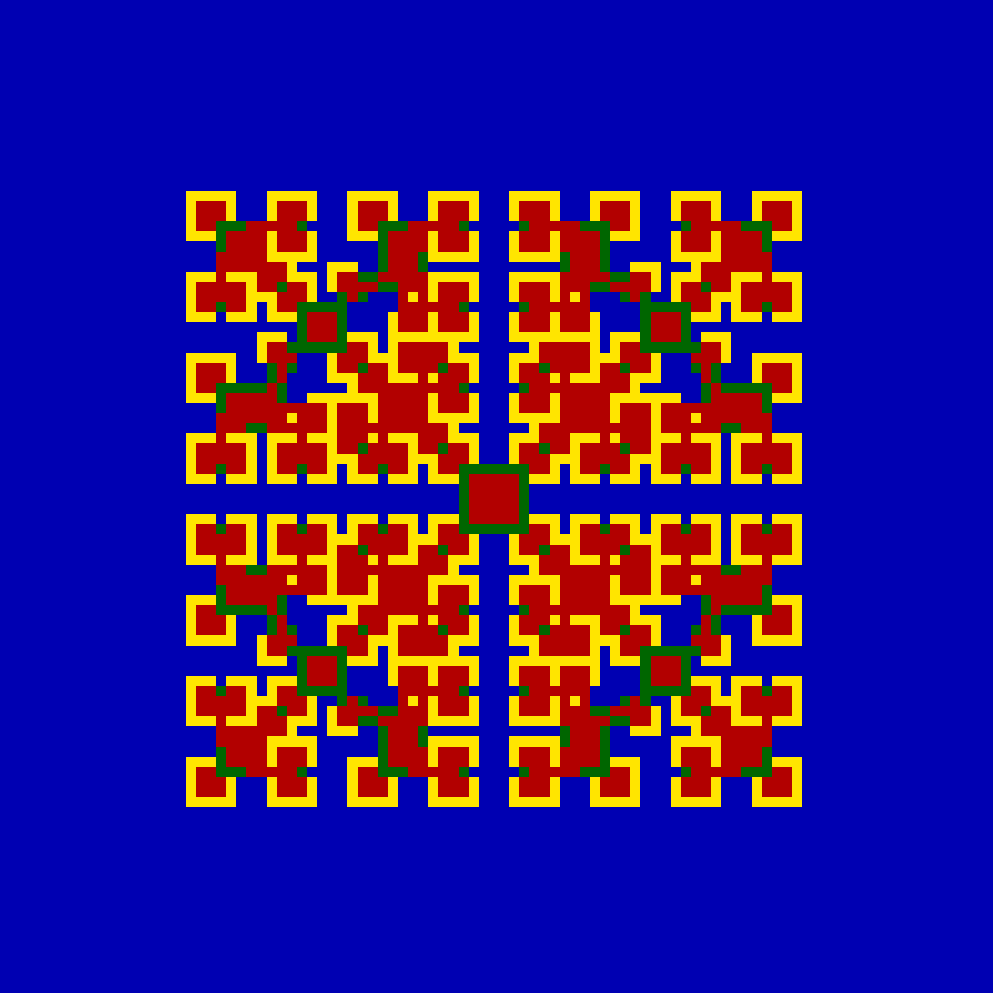
\includegraphics[width=.4\textwidth, angle=0]{./fig/par_99x99_62steps_MSG_haskell.png}
            \caption[]%
            {{\small Parallel Strategy}}    
            \label{fig:par_strat}
        \end{subfigure}
        \vskip\baselineskip
        \begin{subfigure}[b]{0.475\textwidth}   
            \centering 
            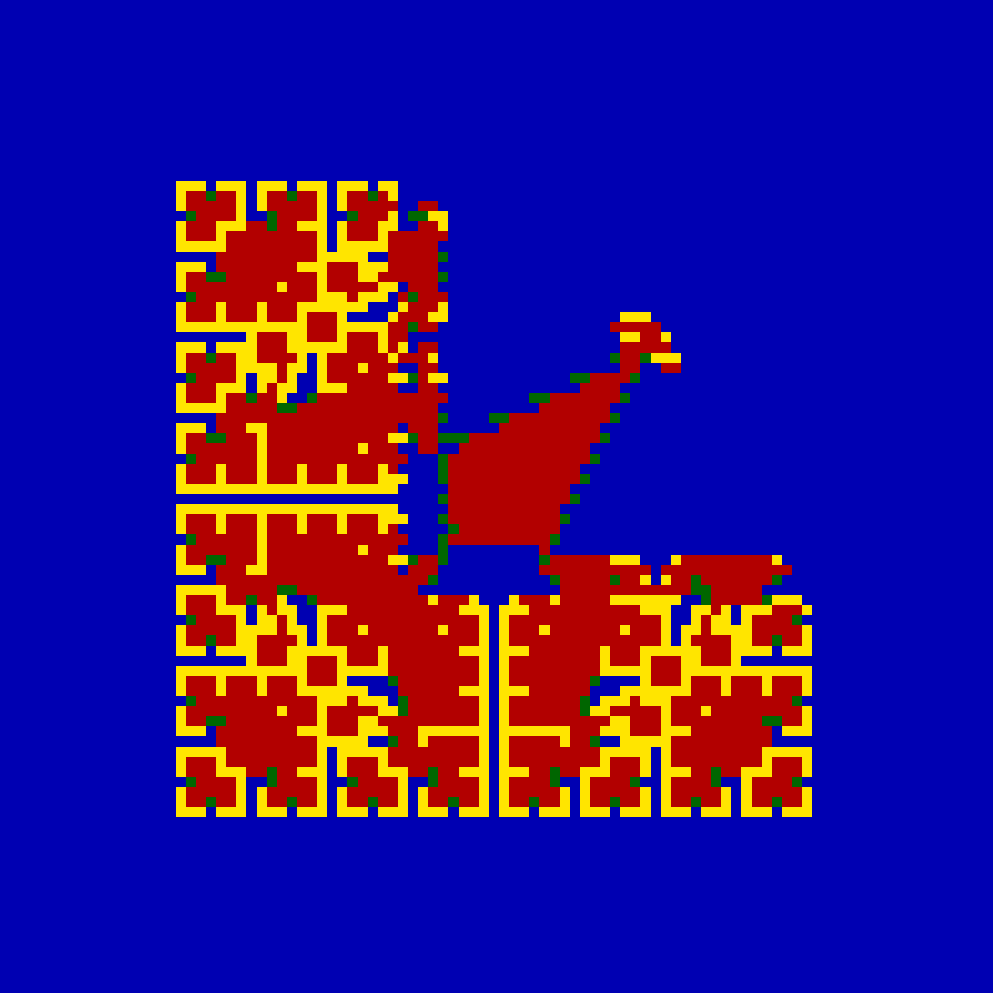
\includegraphics[width=.4\textwidth, angle=0]{./fig/con_99x99_62steps_MSG_haskell.png}
            \caption[]%
            {{\small Concurrent Strategy}}    
            \label{fig:con_strat}
        \end{subfigure}
        \quad
        \begin{subfigure}[b]{0.475\textwidth}   
            \centering 
            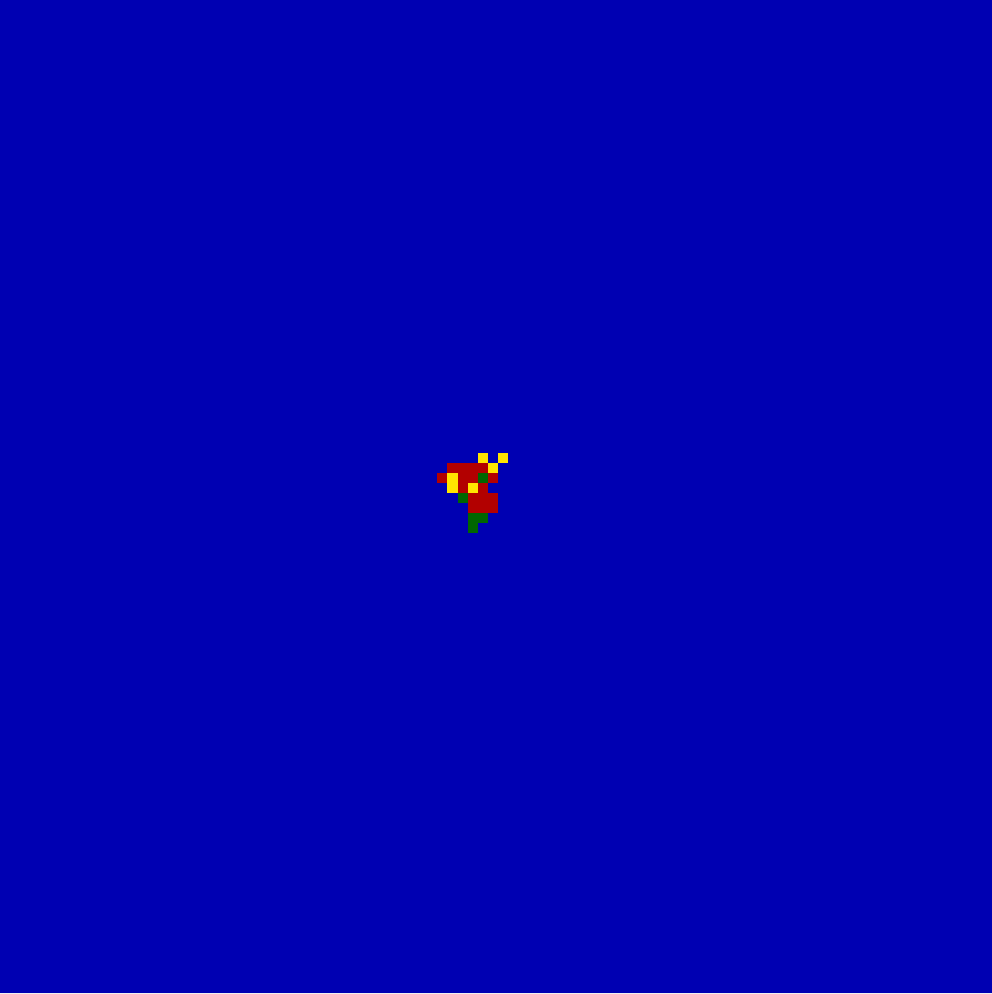
\includegraphics[width=.4\textwidth, angle=0]{./fig/act_99x99_62steps_MSG_haskell.png}
            \caption[]%
            {{\small Actor Strategy}}    
            \label{fig:act_strat}
        \end{subfigure}
        \caption[]
        {\small Haskell implementation of Prisoner-Dilemma game as in \cite{huberman_evolutionary_1993} on a 50x50 grid after 45 steps.} 
        \label{fig:prisoner_strategies}
    \end{figure*}
    
It is immediate clear that, when looking at figure \ref{fig:prisoner_strategies} the update-strategy which reflects the semantics of the model is the Parallel Strategy as all others clearly fail to reproduce the pattern as shown by the results in the original paper. Thus we can imply that only the Parallel Strategy is suitable to simulate this model and that only this strategy is the correct one. \\
The reason why the others fail to reproduce the pattern is due to the non-parallel and unsynchronized way that information spreads through the grid. In the Sequential Strategy the Agents further ahead in the queue play the game earlier and influence the neighbourhood thus Agents in the neighbourhood which play the game later experience an already changed environment and  messages in their queue and act differently based upon these informations. This is not the case in the Parallel version where all Agents play the game on the frozen state of the previous step and the outcome of each Agents game will only be visible in the next step. In the Concurrent and Actor Strategy the Agents run in parallel but changes are visible immediately and concurrently, thus leading to the same non-structural patterns as in the Sequential Strategy. \\
Note that the Concurrent and Actor Strategy produce different results on every run due to the inherent non-deterministic event-ordering introduce by concurrency. Also note that it is not possible to calculate 45 steps for the Actor Strategy as it lacks the Global Synchronization property. To arrive at a relative comparative result we just waited until the first Agent arrives at a local time of 45 and then rendered the result. 

\subsection{Heroes \& Cowards}
We included this model to show that its also possible that results of a model can be invariant under different update-strategies. In Heroes \& Cowards one starts with a crowd of Agents where each Agent is positioned randomly in a continuous 2D-space which is bounded by borders on all sides. Each of the Agents then selects randomly one friend and one enemy (except itself) and decides with a given probability whether the Agent acts in the role of a \textit{Hero} or a \textit{Coward} - friend, enemy and role don't change after the initial set-up. Now the simulation can start: in each step the Agent will move a given distance towards a target point. If the Agent is in the role of a \textit{Hero} this target point will be the half-way distance between the Agents friend and enemy - the Agent tries to protect the friend from the enemy. If the Agent is acting like a \textit{Coward} it will try to hide behind the friend also the half-way distance between the Agents friend and enemy, just in the opposite direction. Note that this simulation is determined by the random starting positions, random friend and enemy selection, random role selection and number of Agents. Note also that during the simulation-stepping no randomness is incurred and given the initial random set-up, the simulation-model is completely deterministic. \\

\begin{figure}
	\centering
  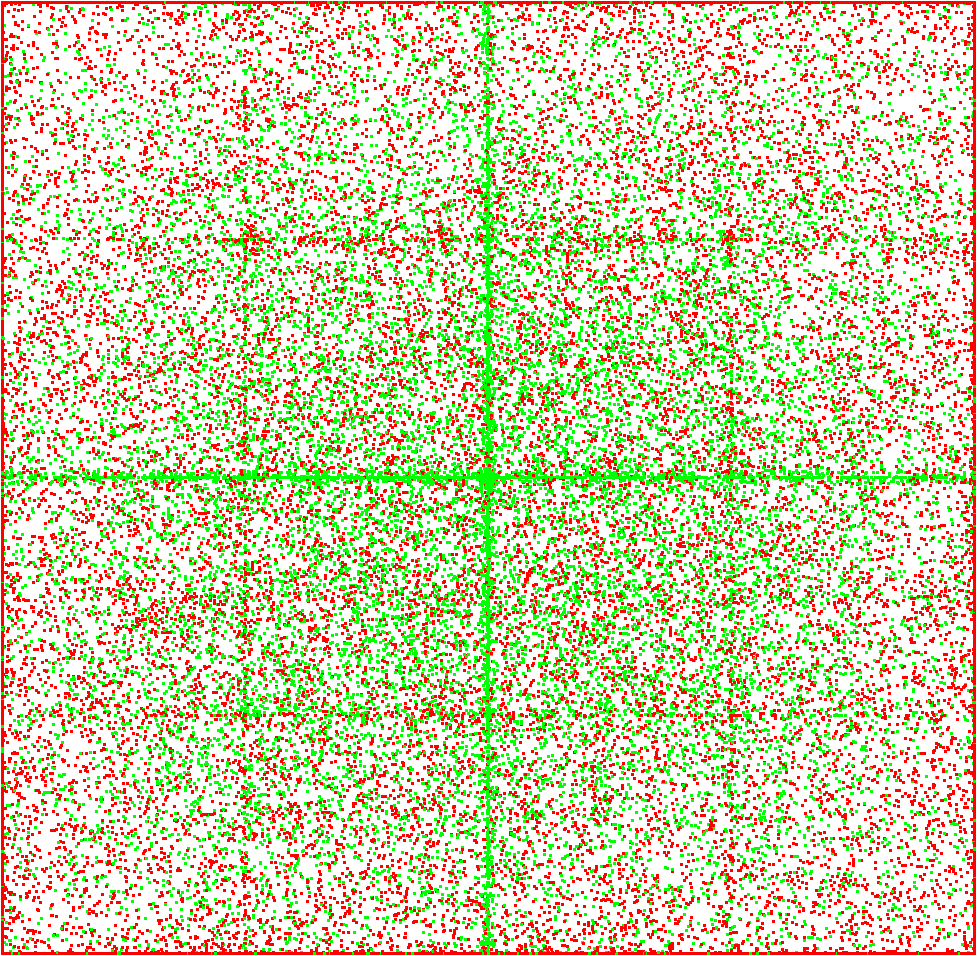
\includegraphics[width=.4\textwidth, angle=0]{./fig/con_HAC_100_000_500steps_haskell.png}
	\caption{Emergent cross-pattern forming in all four update-strategies using 100.000 Agents with 25\% Heroes. Picture taken from running the Concurrent Strategy for 500 steps in our Java implementation.}
	\label{fig:hac_strategies}
\end{figure}

Although the individual Agent-positions of runs with the same configuration differ between update-strategies we experienced the forming of the emergent cross-pattern as seen in figure \ref{fig:hac_strategies} in all four update-strategies. Thus we can conclude that the Heroes \& Cowards model seems to be more robust to the selection of its update-strategy and that its emergent property - the formation of the cross - is stable under differing update-strategies. One would not see a difference between the different strategies thus only one picture was included. Note that to test the Actor Strategy with a this high number of Agents we used our implementation in Scala with Actors as Java is not able to have this high number of threads and our Haskell implementation suffers from performance issues, thus resorting to Scala with Actors. The results were nearly the same there, showing the big green emergent cross-pattern in the center but lacking the smaller red crosses in each section, something we attribute to the local-time of each Agent and the relativity of observing the simulation.